\chapter{Conclusão}

\section{Trabalhos Futuros}

\begin{itemize}
    \item Aperfeiçoar textit{layout da aplicação}
    \item Aprimorar segunça e sincronização da API;
    \item Automatizar ainda mais as tasks para o Docker;
    \item Criar receitas para a aplicação;
    \item Realizar testes funcionais e de integração;
    \item Realizar testes de usabilidade com usuários finais;
    \item Realizar sistema de \textit{log} que informe as ações realizadas pelos usuários;
    \item Realizar um sistema de \textit{backup};
    \item Realizar a funcionalidade para esquecimento de senhas, via e-mail.
    \item Subir a imagem do serviço \textit{web} no Docker Hub;
    \item Utilizar apenas pacotes utilizados pelo SMI-UnB no serviço \textit{web}, visto que a imagem Python 3.5 ocupa muito armazenamento;
\end{itemize}

\section{Cronograma}
Para a realização do cronograma do projeto, figuras \ref{cronograma} \ref{cronograma_2}, utilizou-se a ferramenta \textit{Gantter}. Esta ferramenta aborda como dividiram-se as sprints e atividades realizadas no decorrer do desenvolvimento do SME-UnB.

\begin{figure}[!htpb]
    \centering
    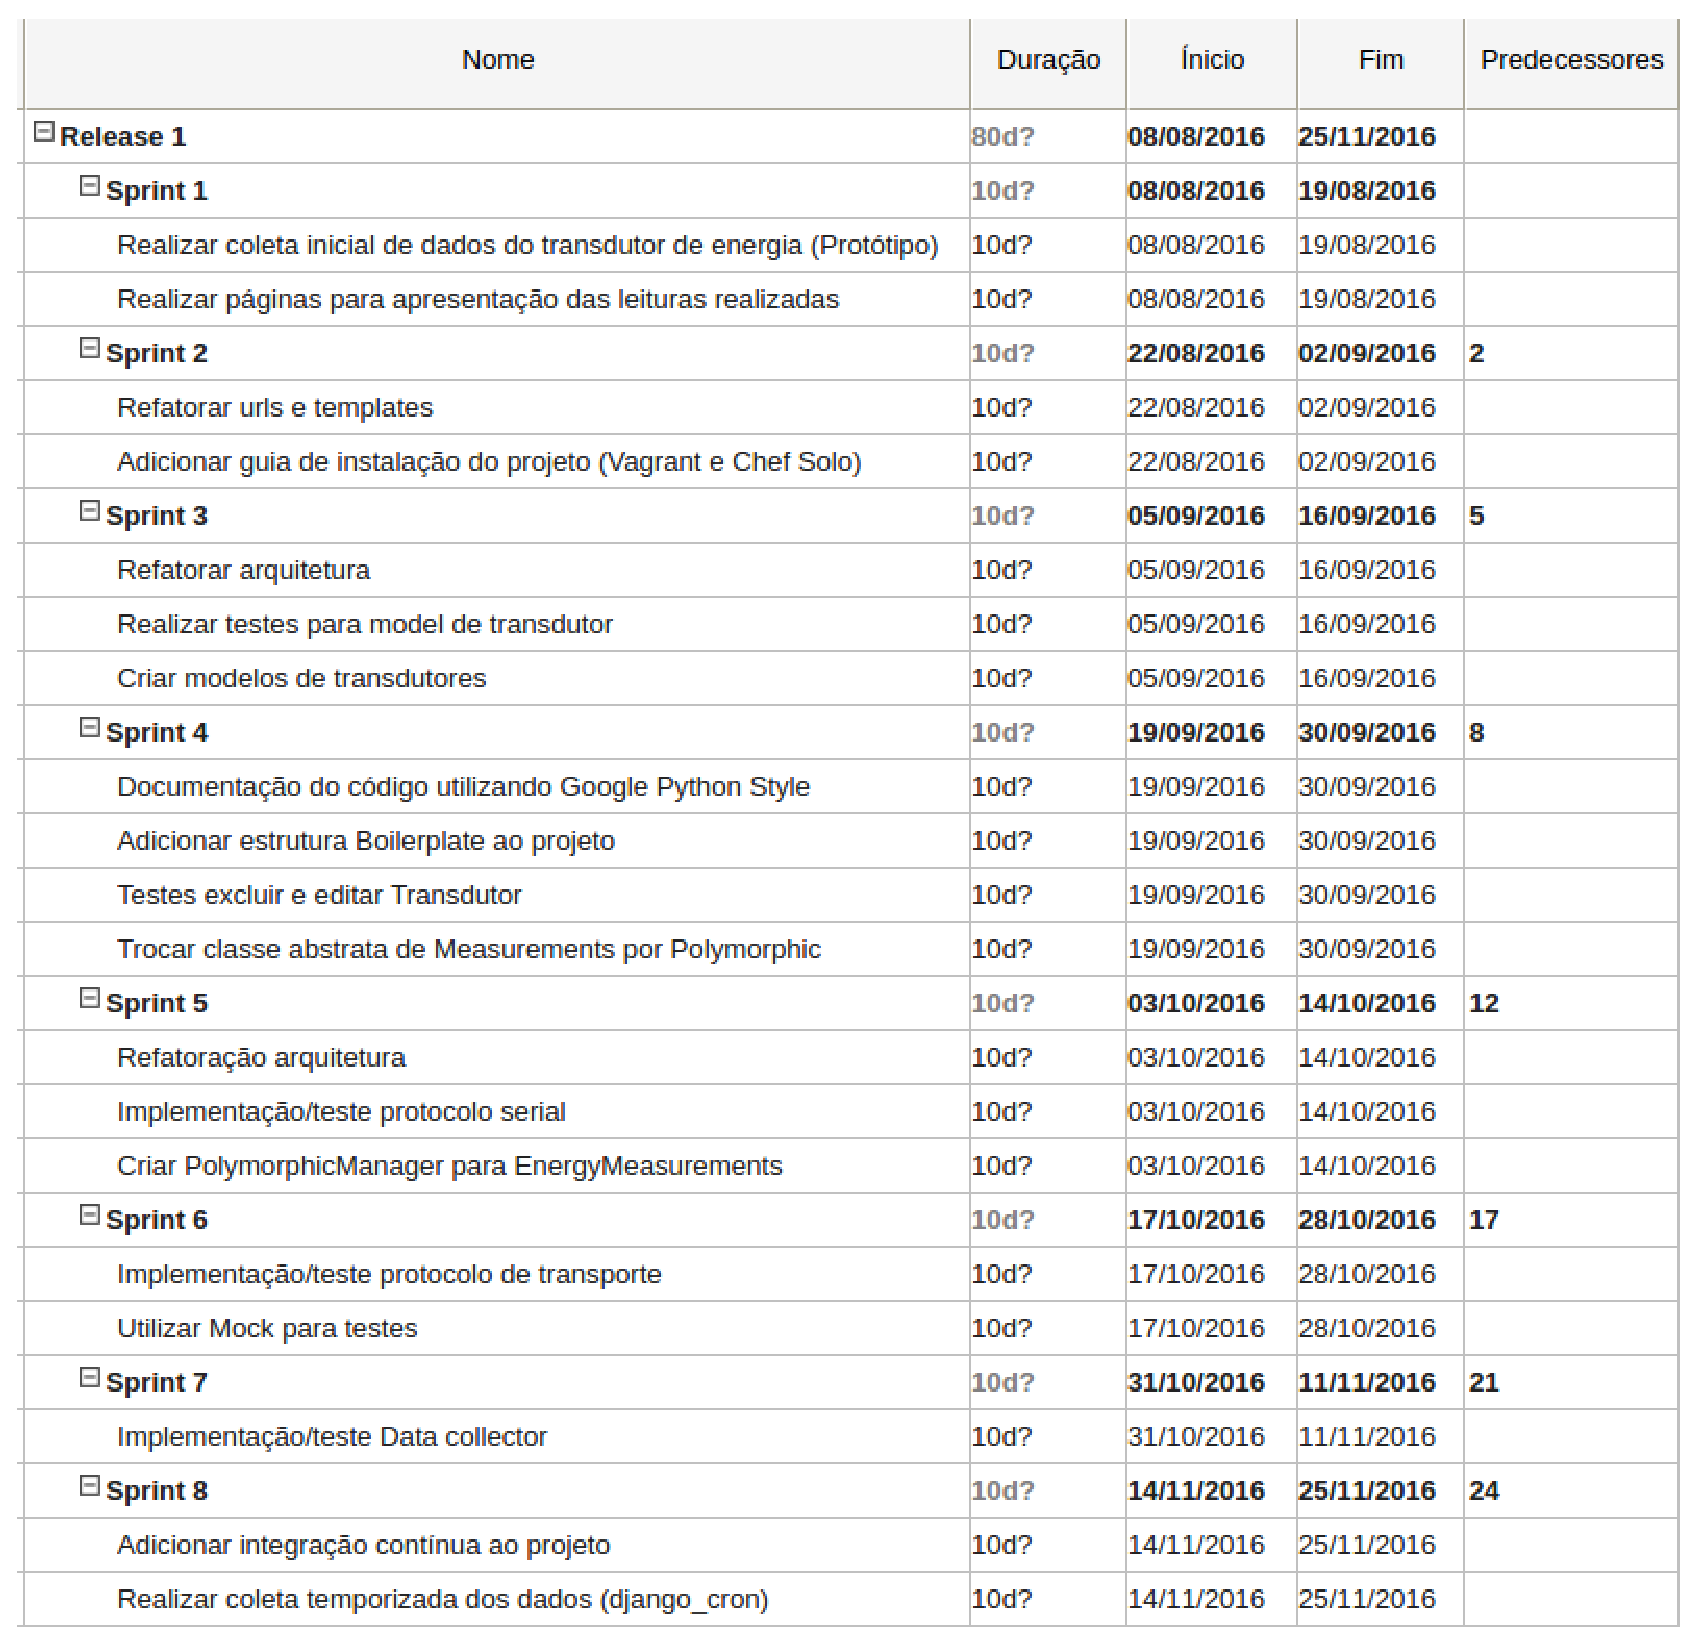
\includegraphics[keepaspectratio=true,scale=0.5]{figuras/cronograma.eps}
    \caption{Cronograma da \textit{release} 1.}
    \label{cronograma}
\end{figure}

\begin{figure}[!htpb]
    \centering
    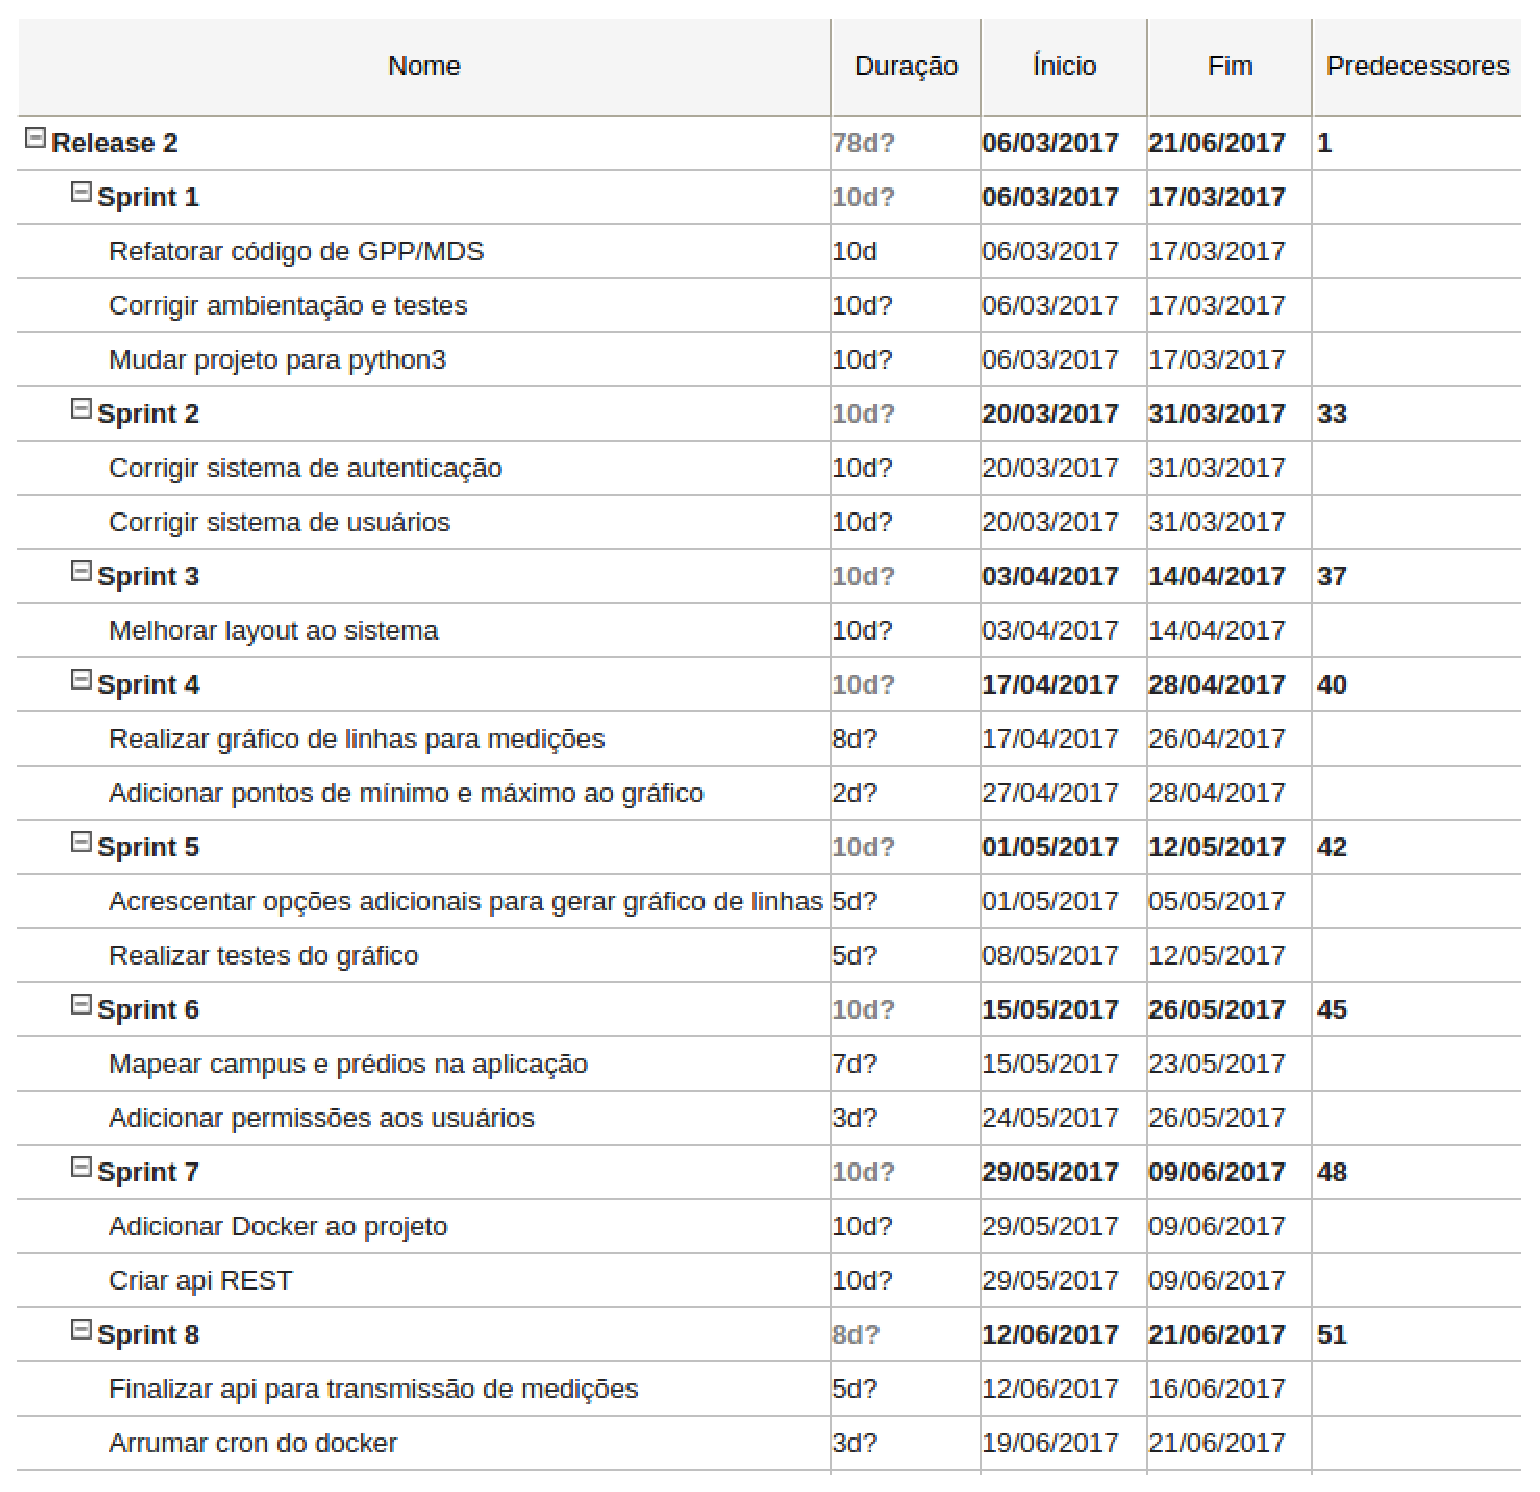
\includegraphics[keepaspectratio=true,scale=0.5]{figuras/cronograma_2.eps}
    \caption{Cronograma da \textit{release} 2.}
    \label{cronograma_2}
\end{figure}